\documentclass{acm_proc_article-sp}

\usepackage{url}
\usepackage{graphicx}

\makeatletter
\def\@copyrightspace{\relax}
\makeatother

\begin{document}

\title{I523: Project: Project\_003: Anomaly detection in network traffic}

\subtitle{\url{https://gitlab.com/cloudmesh\_fall2016/project-003/}}

\numberofauthors{3} 
\author{
\alignauthor
Shweta Bhartia\\
F16-IG-3002\\
       \affaddr{Indiana University}\\
       \affaddr{Bloomington, IN}\\
       \email{sbhartia@umail.iu.edu}
\alignauthor
Pramod Sripada\\
F16-IG-3018\\
       \affaddr{Indiana University}\\
       \affaddr{Bloomington, IN}\\
       \email{ksripada@umail.iu.edu}
\alignauthor
Ramkaushik Nallani\\
F16-IG-3015\\
       \affaddr{Indiana University}\\
       \affaddr{Bloomington, IN}\\
       \email{rnallani@umail.iu.edu}
}

\date{12 December 2016}


\maketitle
\begin{abstract}
Biggest threat in twenty first century is Cyber war. Hackers are trying to intrude into network and hack the systems present in that system thereby stealing the sensitive information. This urges the necessity of detecting anomalous or malicious activities in network so that proper actions can be taken. Anomaly detection in network traffic is challenging task. The anomaly detection classifiers or the anomaly detection models built should be sensitive in not misclassifying normal usage as threats. Too many misclassifications of normal usage results in the ignorance of all the notifications which puts entire system at stake. This paper speaks about data mining techniques devised to detect anomalies in network traffic. Supervised learning methods such as classification can be used in detecting known threats, i.e. the threats which have been experienced in historic data. Anomalies fall under "unknown-unknown" category. Hence supervised techniques cannot be used to find the unknown unknown. Anomaly detection in network traffic is challenging task. Data mining techniques make it possible to search large amount of data for characteristic rules and patterns. In this paper, we build an anomaly classifier using classification methods such as Decision Trees and Random Forest Classifiers, discuss its challenges and then present an anomaly detection algorithm which will be built on K means clustering. Anomaly classifier has the ability to classify earlier patterns but the application of K means technique on training dataset results in the formation of clusters. Corresponding cluster centroids are used as patterns for detection of anomalies in new monitoring data. Proper care has to be taken while building the models which should not be overfitting as small changes in the testing data can render the model useless. We precisely described about the data mining methodology devised for anomaly detection in network traffic in this paper.
\end{abstract}

\terms{Network Intrusion, Computer Security, Network Security, Data Mining, Decision Trees, Random Forest Classifier, K-Means clustering, Apache Spark, HDFS, MLlib}

\section{Introduction}
Advancement in technology and advent of Internet of things has resulted in the huge generation of data. Though storage cost of data is technically reducing day by day, extracting information from vast datasets has really turned into real time challenging problem. Data mining, which strategically amalgamates two different fields namely computer science and statistics is helping in extracting information from the given large sets of raw data. Data scientists find hidden patterns by applying these statistical techniques and forecast future of client's business. Data mining techniques are attracted as they can be applied to any type of dataset to learn about correlations.
Cyber-attacks are growing at very fast pace these days. Most of the attacks attempt to flood a computer with network traffic to gain unauthorized access to any computer. However, if the exploit behavior follows any patterns, they can be detected very easily either by writing simple business rules or through supervised techniques. For instance, if hacker is trying to access services being running in system, he tries accessing ports repeatedly. Hence if a rule is written which throws notification if large number of distinct ports were accessed in short time, attack can be caught. This falls under know known category. But above mentioned techniques cannot be used for detecting unknown unknowns.  Detecting anomalies is the main part in detecting network intrusions. These are connections that are not known to be attacks, but do not resemble connections observed in the past. Hence known supervised methodology can be used only for classifying known attacks and assist the organizations in building rule based systems. Unsupervised learning techniques can be used in detecting unknown attacks, hence this would be a better technique to be used in identifying network intrusion.
Intrusion detection systems process large amount of monitoring data. Some of the most vital Intrusion detection systems are network based Intrusion Detection Systems and Host based Intrusion detection systems. Network based IDS detects harmful packets or packet flows by exploring network monitoring data while host based IDS detects suspicious activities by exploring log files on computer. Advancement of research and development activities in data mining area in late 1990s resulted in the development of better methods for network and host based intrusion detection.
Data mining techniques can be used for detecting anomaly and attack detection by monitoring network data. Anomaly detection can be done in two methods: 1) Classification techniques and 2) Clustering techniques
ML methods are used to train the model to determine what could be the notion of normality. Using classification techniques, certain rules are defined to identify abnormal records. When any of these rules are triggered for a certain connection, it is flagged abnormal. ML based techniques are adaptive, dynamic and requires less human intervention, so they are preferred. Anomaly detection is very intolerant to errors as falsely classifying normal records as attacks or falsely ignoring the attacks renders the system totally useless. Time spent by network security engineer on fixing the anomalies detected is linearly dependent on number of anomalies detected. Hence model should be designed in such a way that anomalies have to be filtered out in best possible way. In this paper, we present an approach for anomaly detection using Decision Tree technique, Random Forest Classifier and K-Means clustering.
Reuters and network monitors which use either Cisco Netflow protocol or IPFIX protocol are the major sources of data related to computer networks. All the data collected constitute flow records. Flow records can be very easily collected as flow monitoring techniques are already deployed in computer networks for administration purposes. Network data mining extracts valuable information from monitoring data which helps in determining dominant characteristics and identifying outliers within the data records. Data mining techniques can also be used to develop rules which are typical for special kind of traffic.
The Dataset used for this project is from the 1998 DARPA Intrusion Detection Evaluation Program which was prepared and managed by MIT Lincoln Labs. Lincoln Labs set up an environment to acquire nine weeks of raw TCP dump data for a local-area network (LAN) simulating a typical U.S. Air Force LAN.  They operated the LAN as if it were a true Air Force environment, but peppered it with multiple attacks. The raw training data is about five million connection records.  Similarly, the test data is around two million connection records. A connection is a sequence of TCP packets starting and ending at some well-defined times, between which data flows to and from a source IP address to a target IP address under some well-defined protocol.  Each connection is labeled as either normal, or as an attack, with exactly one specific attack type. The task is more realistic as it includes specific attack types not in the training data.  This makes the task more realistic. The datasets contain a total of 24 training attack types, with an additional 14 types in the test data only. The dataset is in comma separated value format. We will be performing feature reduction, feature extraction and feature scaling on the dataset for improved performance.
~\cite{www-iacr}
~\cite{www-sciencedirect}
~\cite{www-wikipedia}
~\cite{www-wiki}
~\cite{www-ics-uci}

\section{Exploratory Data Analysis}
\begin{figure}[h]
\includegraphics[width=250]{Distribution-of-types-of-attack.png}
\centering
\caption{Distribution of types of attack}
\label{Distribution of types of attack}
\end{figure}
We have 23 types of attacks. The distribution of types of attacks is shown in the Figure \ref{Distribution of types of attack}. We can observe from the Figure  \ref{Distribution of types of attack} that smurf attack dominates the entire distribution followed by normal  and neptun. The skewness in our dataset is caused by smurf attack.


\begin{figure}[h]
\includegraphics[width=265]{Protocol-Type-vs-Attack.png}
\centering
\caption{Protocol Type vs Attack}
\label{Protocol Type vs Attack}
\end{figure}
The Figure \ref{Protocol Type vs Attack} how attack varies with protocol. Protocol type take three values TCP, UDP and ICMP. In ICMP protocol type, smurf attack is the highest. In TCP protocol type, neptun attack dominates. The users connected through UDP protocol are less prone to the attacks. Hackers are using TCP and ICMP protocol to intrude the network.

\begin{figure*}[h]
\includegraphics[width=\textwidth]{dst-host-count-vs-result.png}
\centering
\caption{Destination host count vs Attack}
\label{Destination host count vs Attack}
\end{figure*}
From the Figure \ref{Destination host count vs Attack}, destination host count have different distributions across all the attacks. Mean of destination host count varying across the attacks depicts its importance. We have observed that destination host count is taking larger values in back attack resulting in high mean.

\begin{figure*}[h]
\includegraphics[width=\textwidth]{Destination-host-srv-count-vs-Attack.png}
\centering
\caption{Destination host srv count vs Attack}
\label{Destination host srv count vs Attack}
\end{figure*}
We have observed in the Figure \ref{Destination host srv count vs Attack} that derived feature destination host count projects different distributions across all the attacks. Normal network connection have high mean value of destination host srv count.

\begin{figure*}[h]
\includegraphics[width=\textwidth]{result-vs-dstbytes.png}
\centering
\caption{Destination bytes vs Attack}
\label{Destination bytes vs Attack}
\end{figure*}
In this Figure \ref{Destination bytes vs Attack}, more destination bytes are observed in normal connection. It is natural tendency of any network to provide access when protocol is normal. Next to normal connection, warezm attack is taking higher values in destination bytes.

\begin{figure*}[h]
\includegraphics[width=\textwidth]{result-vs-srv-count.png}
\centering
\caption{Srv count vs Attack}
\label{srv count vs Attack}
\end{figure*}
The joint distribution of srv count and attack is shown in the Figure \ref{srv count vs Attack}. srv count describes the number of connection to the same service as the current connection in the past two seconds. Srv count of the connection categorised as smurf takes higher values.

\begin{figure*}[p]
\includegraphics[width=\textwidth]{Flag-vs-Attacks.png}
\centering
\caption{Flag vs Attacks}
\label{Flag vs Attacks}
\end{figure*}
The joint distribution of flag and attack is shown in the Figure \ref{Flag vs Attacks}. Flag denotes status of connection and it can either be normal or error. There different sub-categories under error status. In "sf" flag error status, we have highest numbers of smurf attack While in "so" flag error status, neptun attack dominates.

\begin{figure}[h]
\includegraphics[width=265]{Is-Guest-Login-vs-Attacks.png}
\centering
\caption{Is Guest Login vs Attacks}
\label{Is Guest Login vs Attacks}
\end{figure}
We can infer from the Figure \ref{Is Guest Login vs Attacks} that hackers whose attack is categorised as warzerc were logging in as guest. This conveys that hackers were not trying to personify other users while attacking onto the network.

\begin{figure}[h]
\includegraphics[width=265]{result-vs-srcbytes.png}
\centering
\caption{Source bytes vs Attack}
\label{Source bytes vs Attack}
\end{figure}
From the Figure \ref{Source bytes vs Attack}, we inferred that number of bytes from source to destination are more for portsweep probe attack.

\section{Feature Engineering}
Dataset extracted from KDD website includes variety of intrusions which were simulated in a military network environment. Dataset basically consists of numeric and categorical fields. Categorical variables are both ordinal and nominal in nature. Presence of numeric and categorical values makes problem statement very challenging. 
We tackled challenging problem statement through following feature engineering steps:

\begin{enumerate}
\item Log Transformation : Data consists of 41 features. Not all features are equally important.  Before constructing model, feature engineering is vital as it immensely affects the performance of model. While examining the data in python, we found out weird high values for feature "src bytes", "duration", "hot", "num failed logins", "num compromised", "num root" etc and inclusion of those values result in high variance in the model. Hence we have applied logarithmic transformations to all the numeric features which were taking continuous values.
\item Penalization of Multi-collinearity issue : In order to deal the multi collinearity issue in the dataset, we decided to check the correlations between all the numeric features using pearson's correlation . We found very high correlations among couple of features. For instance , "dst host srv rerror rate" and "dst host rerror rate" are positively correlated with 0.98 as correlation coefficient. Figure \ref{Co-linearity check between destination host srv vs destination host} shows the co-linearity between dst host srv rerror rate and dst host rerror rate. Similarly, "dst host srv serror" and "serror rate" are positively correlated with 0.99 as correlation coefficient. Figure \ref{Co-linearity check between destination host srv serror rate vs serror rate} shows the co-linearity between dst host srv serror and serror rate. Both are in fact trying to convey same information regarding target variable. Removal of one variable helps in reducing dimensionality without loss of information. In this way, we have identified highly correlated variables and removed them. This decision has helped in better parameter tuning of algorithm.
\begin{figure}[h]
\includegraphics[width=265]{dst host srv rerror rate vs rerror rate.png}
\centering
\caption{Co-linearity check between destination host srv vs destination host}
\label{Co-linearity check between destination host srv vs destination host}
\end{figure}

\begin{figure}[h]
\includegraphics[width=265]{dst host srv serror rate vs serror rate.png}
\centering
\caption{Co-linearity check between destination host srv vs destination host}
\label{Co-linearity check between destination host srv serror rate vs serror rate}
\end{figure}

\item Identification of Important Features : Given dataset has many features. Identifying best features and designing model on top of them assures low bias and variance to the model constructed. Features selected shouldn't be very less as it might leads to under fitting (High Bias model). Similarly features selected shouldn't be too high as it might lead to over fitting (High Variance model). Hence feature selection is very crucial for proper variance – bias trade off for the model.
We have used the following algorithms for feature selection :

\begin{enumerate}
\item Random Forest classifier technique for feature selection :
We have used "RandomForestClassifier" module from scikit learn package for feature selection. Random Forest can be used as feature ranking method if importance score is assigned to each feature. Fortunately scikit learn package has provided a component called "feature importance" which returns importance score for all the features present in the training dataset. Before calculating feature importance, we have converted all the categorical variables into dummy variables through one hot encoding. We used "entropy" as splitting criteria at each node while constructing each tree of random forest. 
Random forest is combination of trees which are formed by randomly choosing subsets of feature space and randomly selected data points. Random forest helps in selecting important features of the given data set by assigning "importance score" to every feature. Importance score of a feature is calculated in following way:
Random forest puts down the out of bag cases while forming every tree and counts the number of votes cast for the correct class. Now it randomly permutes the values of variable m in the out of bag cases and puts these cases down the tree. Then number of votes for the correct class in the variable-m-permuted out of bag data  are subtracted from the number of votes for the correct class in the untouched out of bag data. The average of this number over all trees in the forest is the raw importance score for variable m.
Random Forest Implementation in Python :
Fortunately, entire process described was taken care by component "feature importance" of random forest classifier of scikit learn package.  Random forest classifier has calculated importance for all features and identified "is host login", "num outbound cmds" as least significant features. We implemented random forest classification method for feature selection in python programming language. We have implemented another algorithm named "boruta" for feature selection. We compare both results. Both algorithms identified "is host login", "num outbound cmds" as least significant features.

\item Boruta algorithm for feature importance:
\begin{figure}[h]
\includegraphics[width=265]{Rplot.png}
\centering
\caption{Rplot}
\label{Rplot}
\end{figure}
Boruta is a feature selection algorithm which works as wrapper algorithm around random forest. Boruta algorithm works in the following way :
1. Extend the information system by adding copies of all variables (the information system
is always extended by at least 5 shadow attributes, even if the number of attributes in
the original set is lower than 5).
2. Shuffle the added attributes to remove their correlations with the response.
3. Run a random forest classifier on the extended information system and gather the
Z scores computed.
4. Find the maximum Z score among shadow attributes (MZSA), and then consider 
every attribute that scored better than MZSA.
5. For each attribute with undetermined importance perform a two-sided test of equality
with the MZSA.
6. Deem the attributes which have importance significantly lower than MZSA as "unimportant" and permanently remove them from the information system.
7. Deem the attributes which have importance significantly higher than MZSA as "important".

Boruta helps in finding all features which are strongly or weakly relevant to decision variable. Boruta follows all relevant feature selection method. All relevant features selection method helps in capturing all the features which are in some circumstances relevant to output variable. In this way, it is different from traditional feature selection algorithms which follows minimal optimal method where they rely on small subset of features which yield minimal error on chosen classifier.
We have implemented boruta algorithm in R programming language. We used boruta package from CRAN repository.
Surprisingly both Boruta and RandomForestClassifier identified "is host login" and  "num outbound cmds" as least significant features.
The output of borutu algorithm can viewed in Figure \ref{Rplot}.
\end{enumerate}
\end{enumerate}

\section{ANALYSIS}
We have implemented supervised technique to train our model. A supervised learning algorithm analyzes the training data and produces an inferred function, which can be used for mapping new examples. An optimal scenario will allow for the algorithm to correctly determine the class labels for unseen instances. This requires the learning algorithm to generalize from the training data to unseen situations in a reasonable way. In supervised technique, we have implemented decision tree, logistic regression, Support Vector Machine, Random Forest Classifier and Extra Tree Classifier.

\begin{enumerate}
\item Decision Tree:
The goal is to create a model that predicts the value of a target variable by learning simple decision rules inferred from the data features.
Decision tree algorithm works in following manner:
\begin{enumerate}
\item Choose the best feature f for the root of the tree
\item Separate the training set into subsets where each subset contains examples that have the same value for f
\item Recursively apply the algorithm on each new subset until all examples have the same class label
\end{enumerate}

We have implemented Decision Tree algorithm in python by importing module named "DecisionTreeClassifier" provided by sklearn.tree PACKAGE. We have implemented decision tree by tuning two parameters Criterion and Splitter by following way in our dataset:
\begin{enumerate}
\item Criterion: "Entropy" came to be the best criterion for splitting the decision tree. Entropy calculates the homogeneity of a sample. If the sample is completely homogeneous the entropy is zero and if the sample is an equally divided it has entropy of one.
\item Splitter: Information gain is calculated after calculating the entropy. The entropy for each branch is calculated. Then it is added proportionally, to get total entropy for the split. The resulting entropy is subtracted from the entropy before the split. The result is the Information Gain, or decrease in entropy. Using the "Best Information Gain" decision tree is further split into subsets.
\end{enumerate}
Initially, we selected criterion as "GINI" and splitter as "best". After carefully examining the sliced part of training set, values of criterion and splitter were chosen as "Entropy" and "Best". With these values for the parameters, we succeeded in classifying dataset of size 10,000 with 99\%-99.5\% accuracy.

\item Support Vector Machine:
In Support Vector Machine (SVM) algorithm, we plot each data item as a point in n-dimensional space (where n is number of features you have) with the value of each feature being the value of a coordinate. Then, we perform classification by finding the hyper-plane that differentiate the two classes very well.

Support Vector Machine (SVM) algorithm works in following manner:
\begin{enumerate}
\item Identify the hyper-planes that segregates the classes well
\item Find the hyper-plane maximizing the distances between nearest data point (either class). This distance is called as "Margin"
\end{enumerate}
We have implemented Support Vector Machine (SVM) algorithm in python by importing module named 'SVC' provided by sklearn.svm PACKAGE. We have implemented SVM by tuning three parameters "kernel", "gamma" and "C" that have higher impact on model performance:
\begin{enumerate}
\item Kernel: The functions that takes low dimensional input space and transform it to a higher dimensional space i.e. it converts not separable problem to separable problem.  It is mostly useful in non-linear separation problem.
\item Gamma: Kernel coefficient for 'rbf', 'poly' and 'sigmoid'. Higher the value of gamma, will try to exact fit the as per training data set i.e. generalization error and cause over-fitting problem.
\item C: Penalty parameter C of the error term. It also controls the tradeoff between smooth decision boundary and classifying the training points correctly.
\end{enumerate}
For better performance, we choose 'rbf' as kernel which is useful for non-linear hyper-plane. We choose C=1.0 and gamma=auto. With these values for the parameters, we succeeded in classifying dataset of size 10,000 with 99\%  accuracy.

\item Logistic Regression :
Logistic regression is a linear classifier which helps in defining a linear boundary that classifies normal records with other attacks. With an intention of building rule based engine for classifying known attacks from the normal connections, we have decided to implement logistic regression. Surprisingly logistic regression performed well in classifying known attacks as "attacks" with accuracy of 0.99. But logistic regression failed badly when test set has unknown attacks. Since anomalies can be both known and unknown, we have decided not to proceed with this algorithm as it is not helping us in identifying or capturing unknown attacks.

\item Extra-Tree Classifier Algorithm:
We have also tried Extra-Tree Classifier for classifying known attacks with normal records. Extra-Tree Classifier also performed extremely well in identifying known attacks as 'attacks" with 99\% accuracy. Extra-Tree Classifier functions are generally cheaper to train from a computational point of view but they grow big. There are times where Extra-Tree Classifier generalizes better than Random Forests. By taking into consideration all these positive aspects into consideration, Extra-Tree Classifier were implemented. We have performed tuning of important parameters of Extra-Tree Classifier and ran on test dataset. Unfortunately, Extra-Tree Classifier too failed in identifying unknown attacks as "attacks". So we have decided to implement unsupervised algorithms for identifying anomalies.
\end{enumerate}

In order to capture unknown attacks, unsupervised techniques are best suited. Supervised techniques cannot filter out unknown attacks. Hence all the rule based engines developed will be useless in identifying anomalies. We have implemented K-means and DBSCAN for unsupervised techniques.
\begin{enumerate}
\item K-Means: K-means on the other hand studies the structure of data and groups similar points accordingly. K-means is one of the simplest unsupervised learning algorithms that solve the well known clustering problem. The procedure follows a simple and easy way to classify a given data set through a certain number of clusters (assume k clusters) fixed a-priori. The main idea is to define k centroids, one for each cluster. These centroids should be placed in a cunning way because of different location causes different result.However, K-means fails miserably in finding non linear shapes structure based on the density.

\begin{figure}[h]
\includegraphics[width=265]{kmeans-moons-2.png}
\centering
\caption{kmeans-moons-2}
\label{kmeans-moons-2}
\end{figure}
The Figure \ref{kmeans-moons-2} is referred from ~\cite{www-dominodatalab}.
K-Means performs poorly on this dataset. The algorithm can not successfully discover the "half-moon" structure, nor can it distinguish the noisy data points from the original data points.K-means algorithm is also not robust to outliers. It tries to assign outliers to any one of the cluster whose centroid is nearest to outlier. Most challenging part for K-means is deciding the value of K. 

\item DBSCAN : In order to identify outliers and perfectly classify them as anomalies, we have decided to use DBSCAN algorithm which is robust to outliers. Density based clustering algorithm has played a vital role in finding non linear shapes structure based on the density. Application of DBSCAN results in perfectly identifying all the points which don't fit in the pattern as anomalies and performs extremely well irrespective of shape of distribution of dataset.
\begin{figure}[h]
\includegraphics[width=265]{dbscan-moons-1.png}
\centering
\caption{dbscan-moons-1}
\label{dbscan-moons-1}
\end{figure}
The Figure \ref{dbscan-moons-1} is referred from ~\cite{www-dominodatalab}.
DBSCAN is a density based clustering algorithm. It groups points that are relatively close to each other into one cluster. DBSCAN algorithm is robust to outliers and helped us in identifying the unknown attacks as outliers. It assigns label "-1" to the outliers.
Unlike K-Means, DBSCAN does not require the number of clusters as a parameter. Rather it infers the number of clusters based on the data, and it can discover clusters of arbitrary shape (for comparison, K-Means usually discovers spherical clusters). Epsilon neighborhood is fundamental to DBSCAN to approximate local density, so the algorithm has two parameters:
\begin{enumerate}
\item Epsilon: The radius of our neighborhoods around a data point p.
\item minPts: The minimum number of data points we want in a neighborhood to define a cluster
\end{enumerate}

Using these two parameters, DBSCAN categories the data points into three categories:
\begin{enumerate}
\item Core Points: A data point p is a core point if Nbhd(p, Epsilon) [Epsilon-neighborhood of p] contains at least minPts; |Nbhd(p,Epsilon)| greater than equal to minPts.
\item Border Points: A data point *q is a border point if Nbhd(q, Epsilon) contains less than minPts data points, but q is reachable from some core point p.
\item Outlier: A data point o is an outlier if it is neither a core point nor a border point. Essentially, this is the "other" class.
\end{enumerate}

DBSCAN algorithm works in following manner :
\begin{enumerate}
\item Pick a point at random that has not been assigned to a cluster or been designated as an outlier. Compute its neighborhood to determine if it's a core point. If yes, start a cluster around this point. If no, label the point as an outlier.
\item Once we find a core point and thus a cluster, expand the cluster by adding all directly-reachable points to the cluster. Perform "neighborhood jumps" to find all density-reachable points and add them to the cluster. If an an outlier is added, change that points status from outlier to border point.
\item Repeat these two steps until all points are either assigned to a cluster or designated as an outlier.
\end{enumerate}

We have implemented DBSCAN algorithm in python by importing modle named "DBSCAN" from package SciKit LEARN PACKAGE. We fixed values to Epsilon and minPts. For better performance, we have randomly selected 10 sets of 10,000 data points and tuned values for Epsilon and minPts parameters by checking the homogeneity of clusters formed for every dataset. After carefully examining the False Positives and False Negatives on the sliced part of training set, values of Epsilon and minPts were chosen as '3' and '5'. With these values for the parameters, we succeeded in classifying known and unknown attacks of dataset of size 10,000 with 99\%-99.5\% accuracy. We have presented the results below:
\end{enumerate}

\section{Description of Clouds}
The Spark program has been run on 3 different clouds. Databricks Community edition cloud, Bigdata-labs.com and Cloudxlab.com
\begin{figure}[h]
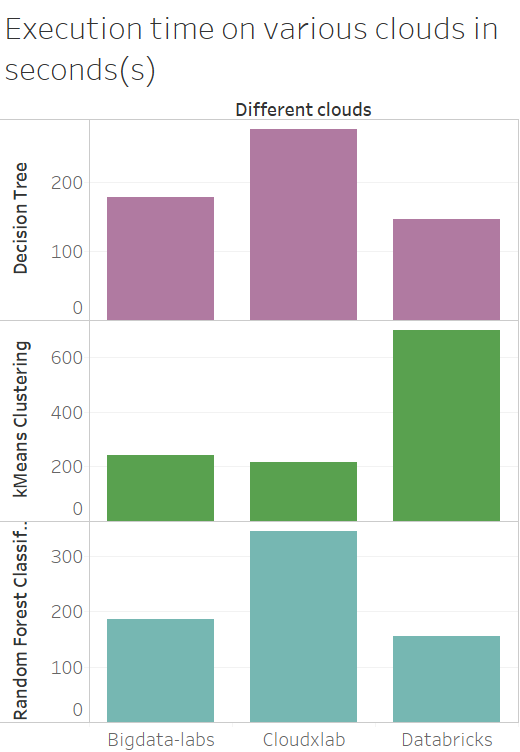
\includegraphics[width=\columnwidth]{Execution time on various clouds in seconds(s).png}
\centering
\caption{Execution time on various clouds in seconds(s)}
\label{Execution time on various clouds in seconds(s)}
\end{figure}
The Figure \ref{Execution time on various clouds in seconds(s)} shows the execution time on the various clouds.

\begin{enumerate}
\item Databricks community edition cloud: Databricks is a public cloud provider that provides Apache Spark clusters. Databricks has been founded by the creators of Apache Spark. Databricks has some unique features that makes it one of the best cloud providers for creating an Apache Spark cluster. It provides an easy way to scale up and scale down the cluster, It provides an interactive notebook for execution of Apache Spark code and provides dashboards for monitoring Spark jobs. 
The community edition of Databricks is a try for free service for students starting to explore Apache Spark, organizations to create Proof of Concept (POC) trying to migrate or create their applications in Apache Spark.
The community edition, gives the user access to a single node Apache Spark cluster. The single node machine contains 3.6 Gigabytes of RAM and 3 cores to process the data in parallel. The data in Apache Spark is stored on the Databricks file system which is a distributed file system, that is built on top of Amazon S3.

\item Cloudxlab: Cloudxlab is a cloud based lab for practicing Apache Hadoop, Apache Spark and related technologies on a real time cluster. The cluster contains 7 nodes each containing 2-8 cores and 8-32 Gigabytes of RAM. The cluster is scaled up depending upon the traffic. Cloudxlab is a paid subscription account and the plans start from 15\$.

\item Bigdata-labs: Bigdata labs is a cloud based lab for practicing Apache Hadoop, Sqoop, Hive and Spark technologies. The cluster contains 5 nodes currently each containing 8 cores and 32 Gigabtes of RAM. The cluster is being upgraded to 9 nodes. The lab has a free subscription through December 31st and offers a value deal for students offering 60\$ for 2 years. 
\end{enumerate}

\section{Results}
After examining  various supervised and unsupervised techniques, we have decided to stick with DBSCAN algorithm which is robust to outliers which are referred as anomalies in our case study.After carefully examining the False Positives and False Negatives on the sliced part of training set, values of Epsilon and minPts were chosen as '3' and '5'. With these values for the parameters, we succeeded in classifying known and unknown attacks of dataset of size 10,000 with 99\%-99.5\% accuracy.We have reported results for three different sliced datasets and tabulated results.

we have randomly selected 10,000 data points which have 8000 data points classified as normal connections and rest are various attacks. Ideally all the attacks need to identified as anomalies by our algorithm. Our algorithm has aptly identified all attacks by either classifying them as outliers (with label -1) or grouped them into single cluster.Results of this dataset are explained in the Figure \ref{Result-1}. But there are 10 normal records which were wrongly grouped with attacks cluster thereby indicating false positive number as 10. Hence error rate for this sample experiment is 0.01 which turned out to be very convincing. In our use case, cost associated with false positives is low compared to false negatives. Our algorithm is not classifying attacks as normal records which is pretty convincing. Yet it has classified 10 normal records as attacks. This might demand network engineer to invest some time in examining normal records. Yet this is not harmful to network as algorithm is aptly identifying all attacks as "attacks" correctly.

we have collected another sample of 10000 records and results for this distribution is depicted by the Figure \ref{Result-2}. All the data points falling in this sample have attack type "smurf" and our algorithm has grouped all these records into single cluster. Error rate for this sample is 0.

We have collected another 10000 points consisting normal and smurf attacks and results for this distribution is depicted by the Figure \ref{Result-3}. Our algorithm has perfectly grouped all smurf records into single cluster (with label 0) and normal records were grouped into two different clusters. As long as homogeneity of cluster is maintained, algorithm is clustering the given data set accurately. But only in Figure \ref{Result-3} normal records were considered as anomalies. Hence error rate for this split is 0.04\%.

We have collected another 10000 data points. results for this distribution is depicted in the Figure \ref{Result-4}.This time, we have records having various attacks. Our algorithm has aptly identified all attacks as "attacks" by either classifying them as outliers(with label -1) or grouping them into separate (all smurf attacks were grouped into single cluster with label 3). However, it has identified 10 normal records as outliers which is error. Hence error rate for this sample is 0.01\%.
\begin{figure}[h]
\includegraphics[width=\columnwidth]{Result-1.png}
\centering
\caption{Result-1}
\label{Result-1}
\end{figure}

\begin{figure}[h]
\includegraphics[width=\columnwidth]{Result-2.png}
\centering
\caption{Result-2}
\label{Result-2}
\end{figure}

\begin{figure}[h]
\includegraphics[width=\columnwidth]{Result-3.png}
\centering
\caption{Result-3}
\label{Result-3}
\end{figure}

\begin{figure}[h]
\includegraphics[width=\columnwidth]{Result-4.png}
\centering
\caption{Result-4}
\label{Result-4}
\end{figure}

\appendix
Shweta Bhartia (F16-IG-3002): Explored data pre-proecssing techniques required to implement supervised algorithms. Implemented min-max scalar technique for numeric features in python.
Implemented data preprocessing steps required for supervised algorithms in spark.
Explored about various supervised algorithms like logistics regression, decision tree, SVM and Extra-tree classifier and implemented all those algorithms in python.
Generated visualizations in tableau.
Ramkaushik Nallani (F16-IG-3015): Explored about data preprocessing techniques like onehot encoding for categorical variables , logarithms transformations to numeric features and implemented in python and spark.
Implemented RandomForest technique and Baruto algorithm for important feature selection and implemented RF in python, Baruto in R programming.
Implemented unsupervised techniques K-means, DBSCAN algorithm in python.
Generated visualizations in matplotlib python
Pramod Sripada (F16-IG-3018): Explored about Spark technology and assisted team members in implementing their developed python scripts in pyspark shell. 
Explored about "Databricks","Big Data labs","CloudX lab" clouds. 
executed scalable code developed in spark on three different clouds and reported run-time.  
Developed spark code for supervised algorithms, K-means technique and integrated with pre-processing spark developed by team members.
Integrated all the python and spark code developed and reported results.
Generated visualizations regarding run-time in tableau and presented in report.

\bibliographystyle{IEEEtran}
\bibliography{references}

\end{document}